\chapter{Curve Elittiche}
Le \textbf{curve elittiche} sono oggetto di studio ben prima che fosse scoperto il loro utilizzo in ambito crittografico, infatti questo venne intuito solo negli anni '80. Questo è grazie al fatto che i punti definiti su una \textbf{curve elittica} (definita su un \textit{campo finito}) formano un \textbf{gruppo} che può essere utilizzato per scopi crittografici. \\
A scopo didattico partiremo da analizzare le \textbf{EC} su $\mathbb{R}$ in modo da poter utilizzare la geometria di esse per ``intuire'' il significato di certe operazioni. Su campi finiti invece si perde la geometria definita in $\mathbb{R}$ ma rimane l'algebra che è indipendente dal campo sottostante.
\\ \newline
Un \textbf{campo} (\textbf{field}) è un insieme \textit{F} su cui sono definite due operazioni: l'addizione e la moltiplicazione \textbf{logica} che indicheremo con: $\{+, \times\}$. Per esplicitare il campo con le sue operazioni si usa la notazione $(F, +, \times)$, tuttavia quando le operazioni sono ben chiare nel contesto lo indicheremo unicamente con il gruppo. Affinche \textit{F} sia un \textbf{campo} bisogna che sia un \textbf{gruppo} rispetto ad entrambe le operazioni contemporaneamente e, in aggiunta, deve anche valere la proprietà \textbf{distributiva} della somma rispetto al prodotto. Naturalmente, per l'\textit{elemento neutro dell'addizione} non è richiesto un inverso moltiplicativo. Razionali, reali e complessi sono ben noti campi \textbf{infiniti}. \\ 
Nell'informatica invece trovano applicazione i \textbf{campi finiti}, detti anche \textbf{\textit{Galois Field}} (\textbf{\textit{GF}}). Il più semplice al quale si può pensare è \textbf{\textit{GF(2)}}, ovvero l'insime $\{0, 1\}$ sul quale sono definite le operazioni $\{\oplus, \land \}$.

\section{Campi Finiti}
Come abbiamo anticipato il \textbf{campo finito} più semplice è il \textbf{\textit{GF(2)}}. Se definiamo \textit{p} come un numero primo, l'insieme $\mathbb{Z}_p$ con le operazioni modulari: $\{+_p, \times_p\}$ definete su di esso formano un campo:
\begin{center}
    $GF(p) = (\mathbb{Z}_p, +_p, \times_p)$
\end{center}
Esistono anche \textbf{campi finiti} di \textit{n} elementi se e solo se $n = p^k, \;\; k \geq 1$, che verrà indicato con \textbf{GF($p^k$)}, ovviamente nel caso in cui $k = 1$ avremo l'ugualianza:
\begin{center} 
    $GF(p^k) = \mathbb{Z}_p \iff k = 1$
\end{center}
Se, invece, $k > 1$ il campo è costituito dai \textbf{polinomi} di grado \textbf{minore di \textit{k}} con coefficiente in $\mathbb{Z}_p$, le operazioni su questi \textbf{campi} sono effettuate \textbf{modulo} un \textbf{polinomio di grado \textit{k} irriducibile} su $\mathbb{Z}_p$. \\
Consideriamo come esempio $GF(3^2)$ avremo che quindi i suoi elementi saranno composti dai polinomi di grado al massimo \textit{1} con i coefficienti che saranno modulo \textit{3}:
\begin{center}
    $GF(3^2) = \{1, 2, 3, x, x + 1, x + 2, 2x, 2x + 1, 2x + 2\} \Rightarrow x^2 + 1$ 
\end{center}
In questo caso possiamo utilizzare come \textbf{polinomio irriducibile} $x^2 + 1$ e quindi dovremo prendere il resto della divisione intera per il \textit{polinomio irriducibile}. \\
Definiamo un po' di termini: l'\textbf{ordine} di un campo finito è il numero dei suoi elementi, la \textbf{caratteristica} di un campo finito è il numero di volte che dobbiamo sommare un elemento a \textit{0} prima di ottenere di nuovo \textit{0}, in un campo di \textit{ordine $p^k$} la \textit{caratteristica} è \textit{p}. Se la somma non raggiunge mai lo \textit{0}, cosa che accade nei campi infiniti, allora la \textit{caratteristica} è \textit{0}. \\
\textbf{Chiusura Algebrica}: un campo \textit{F} si dice \textbf{algebricamente chiuso} se ogni polinomio univariato (di ordine maggiore di \textit{0}, cioè non costanti) ha uno zero in \textit{F}.

\newpage
\section{Curva Elittica}
Consideriamo \textbf{EC} già poste nella forma normalizzata di \textbf{\textit{Weierstrass}}, ovvero diremo che una curva elittica \textbf{E} su un campo \textit{F} è una curva cubica su \textit{F} definita dall'equazione:
\begin{center}
    $y^2 = x^3 + a \cdot x + b, \qquad a, b \in F$
\end{center}
Se $(\overline{x}, \overline{y})$ soddisfano l'equazione allora anche $(\overline{x}, -\overline{y})$ soddisfa l'equazione $\Rightarrow$ \textbf{simmetrico} rispetto all'\textbf{asse x}.
\begin{center}
    $P = (\overline{x}, \overline{y})\;\;\Rightarrow\;\;-P = (\overline{x}, -\overline{y})$
\end{center}
In crittografia sono di interesse le \textbf{curve lisce}, anche dette \textbf{smooth}, avvero curve in cui le derivate parziali non si annullano simultaneamente $\Rightarrow$ in ogni punto esiste una e una sola tangente:
\begin{center}
    \begin{math}
        \begin{aligned}
            \frac{d}{dy}E(x, y) &= \frac{d}{dy}(y^2 - x^3 - ax - b) = 2y \\
            &\Rightarrow \text{ che si annulla solo per } y = 0 \\
            \frac{d}{dx}E(x, y) &= \frac{d}{dx}{y^2 - x^3 - ax - b} = 3x^2 + a \\
        \end{aligned}
    \end{math}
\end{center}
Avremo che i punti che rendono la \textbf{curva non smooth} soddisfano \textbf{simultaneamente}:
\begin{center}
    \begin{math}
        \begin{cases}
            x^3 + ax + b = 0 \\
            3x^2 + a = 0    
        \end{cases}
    \end{math}
\end{center}
Se poniamo $x = 0$ si vede che la curva \textbf{non è liscia} se e solo se $a = b = 0$, se $a = 0, b \neq 0$ le due equazioni non si possono annullare contemporaneamente e quindi la curva sarà \textbf{smooth}. Avremo che, ovviamente, nel caso in cui $y^2 = x^3$ la curva non sarà liscia. In conclusione le curve non lisce vanno cercate ponendo $a < 0 \land x \neq 0$.
\begin{center}
    \begin{math}
        \begin{cases}
            x^3 + ax + b = 0 \\
            3x^2 + a = 0
        \end{cases}
        \Rightarrow
        \begin{cases}
            3 \cdot (x^3 + ax + b) = 3 \cdot 0 \\
            x \cdot (3x^2 + a) = x \cdot 0
        \end{cases}
        \Rightarrow
        \begin{cases}
            3x^3 + 3ax + 3b = 0\;( - )\\
            3x^3 + ax = 0
        \end{cases}
        \Rightarrow 
        \begin{cases}
            2ax + 3b = 0 \\
            3x^2 + a = 0
        \end{cases}
        \Rightarrow
        \begin{cases}
            x = - \frac{3b}{2a} \\
            \frac{27b^2 + 4a^3}{4a^2} = 0
        \end{cases}
    \end{math}
\end{center}
Avremo quindi ottenuto che la curva \textbf{non è liscia} se e solo se la quantità $\Delta = 27b^2 + 4a^3$ è nulla, questa quantità viene anche definita \textbf{discriminante della curva}, e nel caso avremo il punto di \textbf{singolarità} in $P(- \frac{3b}{2a}, 0)$. Normalmente una \textbf{EC} nella forma di \textit{Weierstrass} è definita dai parametri $(a, b)$ e quindi si indica con $E_{(a,b)}$.

\subsection{Curve Elittiche Smooth}

\begin{figure}[h]
    \centering
    \begin{minipage}[t]{0.45\textwidth}
        \centering
        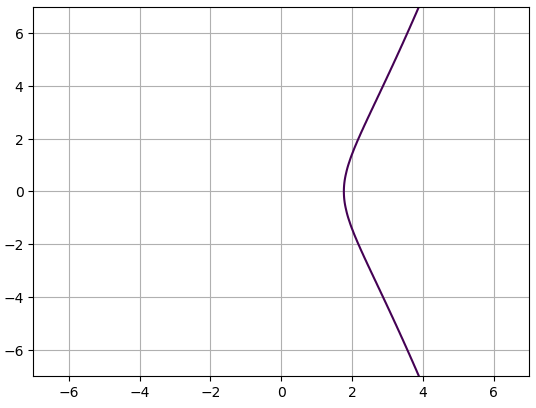
\includegraphics[width=\textwidth, valign=c]{ec_liscia_1.png}
        \caption{$E_{(-2, -2)}$}
    \end{minipage}
    \hfill
    \begin{minipage}[t]{0.45\textwidth}
        \centering
        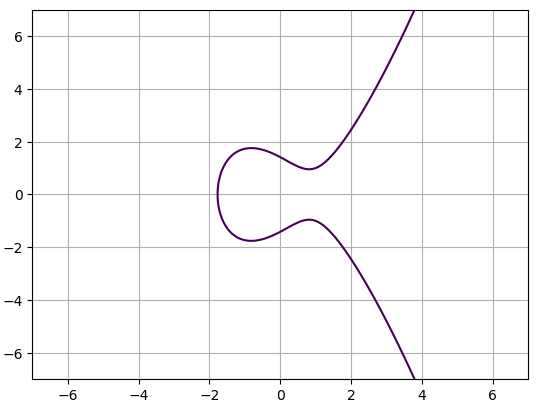
\includegraphics[width=\textwidth, valign=c]{ec_liscia_2.png}
        \caption{$E_{(-2, 2)}$}
    \end{minipage}\par
    \vskip\floatsep
    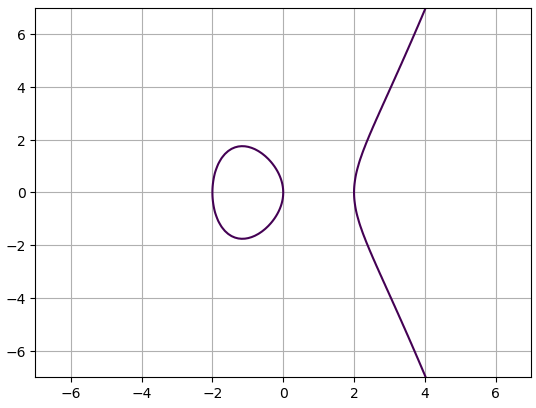
\includegraphics[width=0.45\textwidth]{ec_liscia_3.png}
    \caption{$E_{(-4, 0)}$}
\end{figure}

\newpage
\subsection{Curve Elittiche non Smooth}

\begin{figure}[h]
    \centering
    \begin{minipage}[t]{0.45\textwidth}
        \centering
        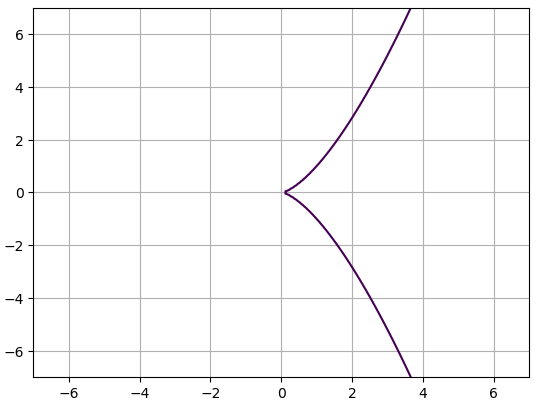
\includegraphics[width=\textwidth, valign=c]{ec_nonliscia_1.png}
        \caption{$E_{(0, 0)}$}
    \end{minipage}
    \hfill
    \begin{minipage}[t]{0.45\textwidth}
        \centering
        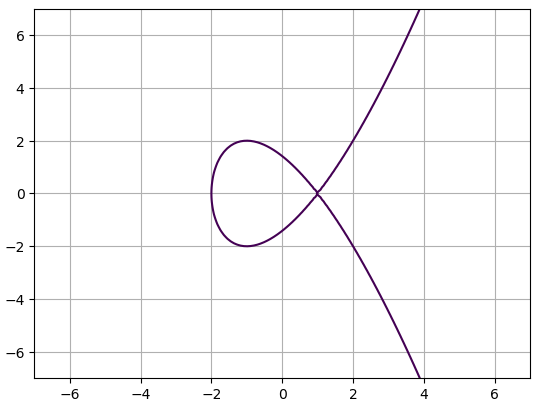
\includegraphics[width=\textwidth, valign=c]{ec_nonliscia_2.png}
        \caption{$E_{(-3, 2)}$}
    \end{minipage}
\end{figure}

\section{Operazioni Geometriche su una Curva}
\textbf{Intersezioni con una retta}: definiamo \textit{R} una retta di equazione $y = mx + q$ e una curva \textit{E} di equazione $y^2 = x^3 + ax + b$, avremo quindi le coordinate \textit{x} di intersezione tra \textit{R} e \textit{E} ($E \cup R$) definite implicitamente dagli zeri di $E(x, y) = y^2 - x^3 - ax - b$.
\begin{center}
    \begin{math}
        \begin{aligned}
            (mx + q) ^ 2 &=& x^3 + ax + b \\
            mx^2 + q^2 + 2mxq &=& x^3 + ax + b \\
            x^3 + ax + b - mx^2 - q^2 - 2mxq &=& 0 \\
            E(x, y) &=& x^3 - mx^2 - (a - 2mq) \cdot x - q^2
        \end{aligned}
    \end{math}
\end{center}
Si tratta di un polinomio \textbf{cubico} e sappiamo che, nel campo reale, esso deve avere \textbf{uno} o \textbf{tre zeri reali} (se ne ha uno solo, gli altri due zeri sono \textbf{complessi coniugati}). \\
Andando a studiare i casi particolari avremo:
\begin{center}
    \begin{math}
        E(x, y) =
        \begin{cases}
            x^3 + ax + b - q^2 \qquad m = 0 \\
            y^2 - c^3 - ac - b \qquad R: x = c 
        \end{cases}
    \end{math}
\end{center}
Su un \textbf{campo finito \textit{F}} non è assolutamente detto che un'equazione $P(x) = 0$, dove \textit{P} è un polinomio a coefficienti in \textit{F} di \textbf{grado dispari}, abbia almeno una soluzione in \textit{F}. È importante notare che nel caso in cui $F = \mathbb{Z}_p$ ha due zeri in \textit{F}, allora anche il terzo zero è in \textit{F}, tenendo presenti le molteplicità degli zero. Nel caso in cui, invece il polinomio a grado 2, ovvero è una \textbf{retta verticale} che incrocia la curva in \textbf{due punti} sarà necessario considerare un ulteriore punto di intersezione, che apparterrà ad un'estensione di F (reale o finito).

\begin{center}
    \textbf{\textit{m = 0}} $\Rightarrow$ \textbf{rette orizzontali}
    \begin{figure}[h]
        \centering
        \begin{minipage}[t]{0.45\textwidth}
            \centering
            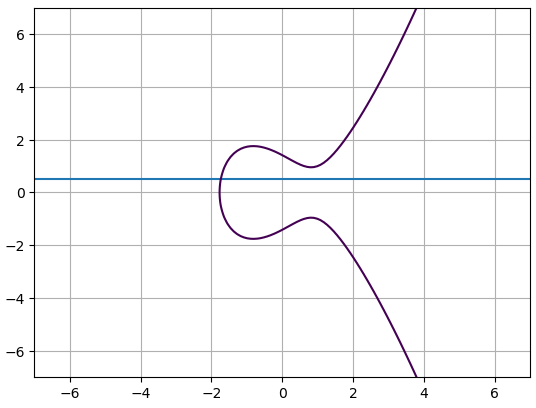
\includegraphics[width=\textwidth, valign=c]{m0_p1.png}
            \caption{$E_{(-2, 2)} \cup q = 0.5$}
        \end{minipage}
        \hfill
        \begin{minipage}[t]{0.45\textwidth}
            \centering
            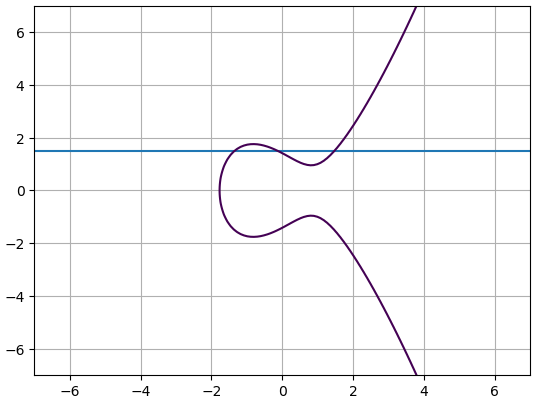
\includegraphics[width=\textwidth, valign=c]{m0_p3_1.png}
            \caption{$E_{(-2, 2)} \cup q = 1.5$}
        \end{minipage}\par
        \vskip\floatsep
        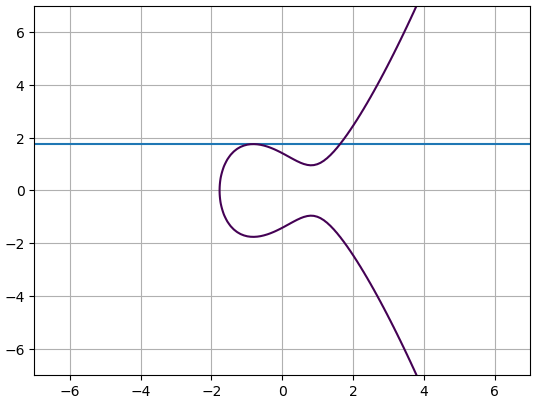
\includegraphics[width=0.45\textwidth]{m0_p3_2.png}
        \caption{$E_{(-2, 2)} \cup q = 1.7427$}
    \end{figure}
\end{center}
\begin{itemize}
    \item Nella \textit{Figura 6.6} abbiamo che la retta interseca una sola volta la curva.
    \item Nella \textit{Figura 6.7} abbiamo che la retta interseca la curva in tre punti, tutti con molteplicità \textit{1}.
    \item Nella \textit{Figura 6.8} abbiamo che la retta interseca 2 volte la curva, il primo punto altro non è che il punto di intersezione tra la curva e la tangente della curva in quel punto, che quindi avrà molteplicità \textit{2} e l'altro invece appartiene alla curva e quindi ha molteplicità \textit{1}
\end{itemize}

\begin{center}
    {\textbf{\textit{m = $\infty$}} $\Rightarrow$ \textbf{rette verticali}
    \begin{figure}[h]
        \centering
        \begin{minipage}[t]{0.45\textwidth}
            \centering
            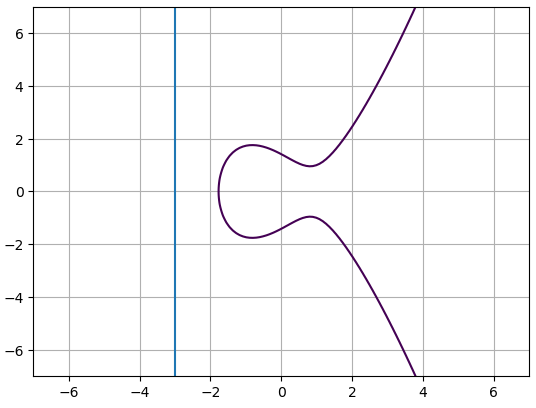
\includegraphics[width=\textwidth, valign=c]{m_inf_p0.png}
            \caption{$E_{(-2, 2)} \cup m = \infty, q = -3$}
        \end{minipage}
        \hfill
        \begin{minipage}[t]{0.45\textwidth}
            \centering
            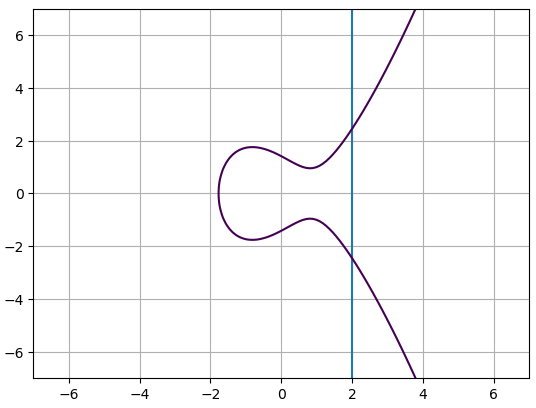
\includegraphics[width=\textwidth, valign=c]{m_inf_p2_1.png}
            \caption{$E_{(-2, 2)} \cup m = \infty, q = 2$}
        \end{minipage}\par
        \vskip\floatsep
        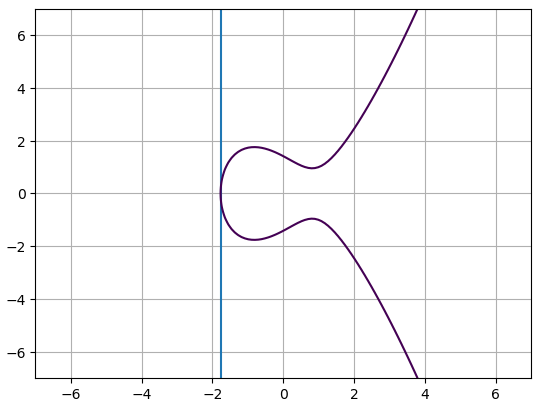
\includegraphics[width=0.45\textwidth]{m_inf_p2_2.png}
        \caption{$E_{(-2, 2)} \cup m = \infty, q = -1.76$}
    \end{figure}}
\end{center}
\begin{itemize}
    \item Nella \textit{Figura 6.9} abbiamo che la retta non interseca la curva.
    \item Nella \textit{Figura 6.10} abbiamo che la retta interseca la curva in due punti, tutti con molteplicità \textit{1}.
    \item Nella \textit{Figura 6.11} abbiamo che la retta interseca la curva come tangente di essa, quindi il punto avrà molteplicità \textit{2}.
\end{itemize}

\newpage
\begin{center}
    \textbf{\textit{m > 0, finito}} $\Rightarrow$ \textbf{rette oblique}
    \begin{figure}[h]
        \centering
        \begin{minipage}[t]{0.45\textwidth}
            \centering
            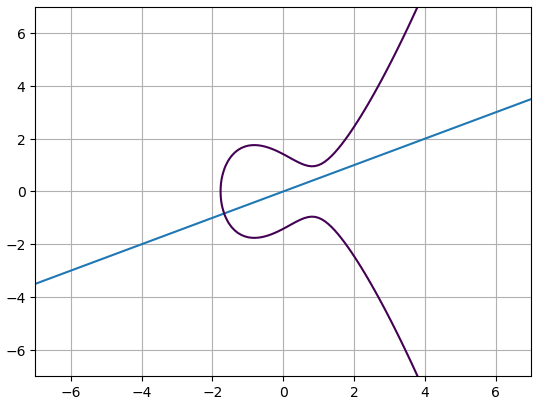
\includegraphics[width=\textwidth, valign=c]{m_p1.png}
            \caption{$E_{(-2, 2)} \cup m = 4$}
        \end{minipage}
        \hfill
        \begin{minipage}[t]{0.45\textwidth}
            \centering
            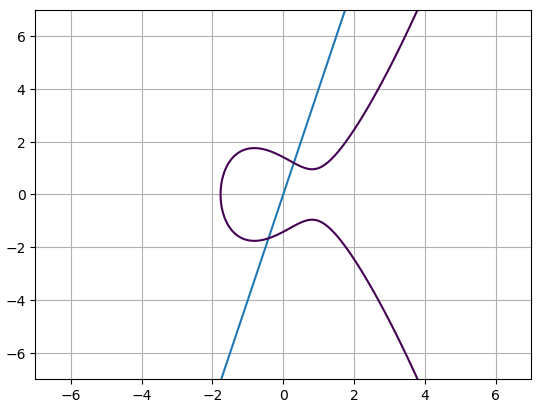
\includegraphics[width=\textwidth, valign=c]{m_p3_1.png}
            \caption{$E_{(-2, 2)} \cup m = 0.5$}
        \end{minipage}
        \begin{minipage}[t]{0.45\textwidth}
            \centering
            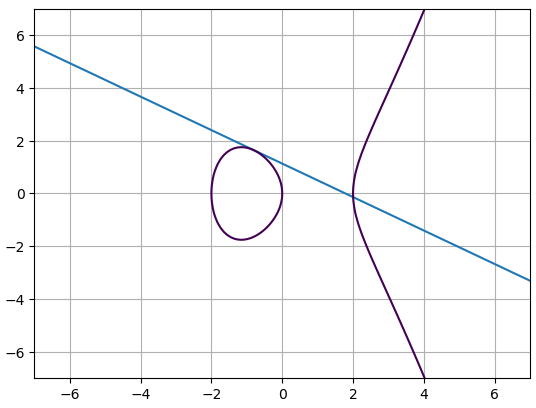
\includegraphics[width=\textwidth, valign=c]{m_p3_2.png}
            \caption{$E_{(-2, 2)} \cup m = -0.741, q = 1.416$}
        \end{minipage}
        \hfill
        \begin{minipage}[t]{0.45\textwidth}
            \centering
            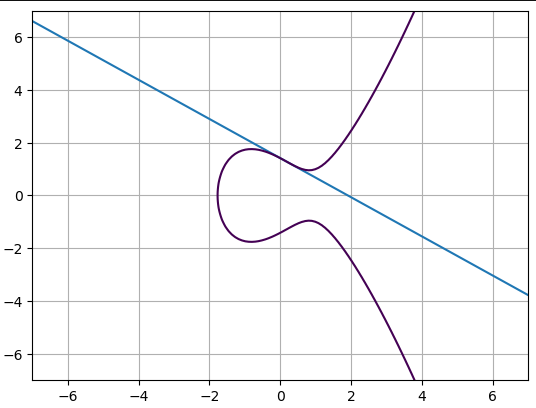
\includegraphics[width=\textwidth, valign=c]{m_p3_3.png}
            \caption{$E_{(-2, 2)} \cup m = -0.634, q = 1.132$}
        \end{minipage}
    \end{figure}
\end{center}
\begin{itemize}
    \item Nella \textit{Figura 6.12} avremo che la retta interseca la curva in un unico punto.
    \item Nella \textit{Figura 6.13} in questo caso avremo che la retta interseca, visivamente, la curva in soli due punti, entrmabi con molteplicità \textit{1}, ma sappiamo che siccome la curva \textit{E}, al crescere di \textit{x}, si comporta come $x^{\frac{3}{2}}$, quindi con velocità \textit{superlineare}, sappiamo che sarà presente un altro punto di intersezione con molteplicità \textit{1}.
    \item Nella \textit{Figura 6.14}: abbiamo che la retta interseca 2 volte la curva, il primo punto altro non è che il punto di intersezione tra la curva e la tangente della curva in quel punto, che quindi avrà molteplicità \textit{2} e l'altro invece appartiene alla curva e quindi ha molteplicità \textit{1}
    \item Nella \textit{Figura 6.15}: in questo caso la retta interseca la curva in un unico punto, che però essendo un punto di \textbf{flesso} della curva ha molteplicità \textit{3}.
\end{itemize}
Abbiamo definito che ai fini \textbf{crittografici} i casi di interesse sono quelli in cui sono presenti \textbf{3 punti di intersezione}. È infatti possibile definire un \textbf{gruppo} costituito proprio dai punti sulla curva. Nel caso di rette \textbf{verticali} ovvero con $m = \infty$ sono presente unicamente due punti di intersezione sulla curva. Detta in maniera discorsiva, vorremmo che quando sono presenti due intersezioni ce ne fosse \textbf{sempre} una terza, mentre invece se non ci sono intersezioni o ce n'è una sola \textbf{non sono rilevanti}. \\
La soluzione più semplice è quella di considerare un punto ``extra'', che indicheremo con $\mathcal{O}$, detto anche \textbf{Punto all'Infinito}. Il punto viene aggiunto ad \textit{F} ed è inteso far parte di qualsiasi curva \textit{E} su \textit{F}. Come vedremo $\mathcal{O}$ fungerà da \textbf{elemento neutro} dell'operazione di gruppo. \\
Proprietà di $\mathcal{O}$ :
\begin{itemize}
    \item qualsiasi \textbf{retta verticale} interseca \textit{E} in $\mathcal{O}$ con molteplicità \textit{1}, ne consegue che se \textit{R} ha già due intersezioni con \textit{E} il \textbf{punto all'infinito} costituirà il terzo punto di intersezione.
    \item nessuna retta con di equazione $y = mx + q$ con $m > 0$ finito interseca il punto $\mathcal{O}$.
    \item nel punto $\mathcal{O}$ la curva ha tangente \textit{t}. Si suppone che che \textit{t} abbia come unica intersezione con la curva proprio il punto $\mathcal{O}$ con molteplicità \textit{3}.
    \item $\mathcal{O}$ coincide con il suo opposto $-\mathcal{O}$.
    \item con l'introduzione del punto all'infinito, \textit{E} gode della seguente proprietà: \textbf{Sia \textit{R} una retta definita in \textit{F}, se \textit{R} ha due punti di intersezione in \textit{F} con la curva \textit{E}, allora ha anche un terzo punto di intersezione in \textit{F}}.
\end{itemize}

\newpage
\textbf{Addizione su Curva Elittica} \\
La somma di due punti $A, B \in E$ è definita come $A + B = -C$ ovvero la somma di \textit{A} e \textit{B} è il punto simmetrico al terzo punto di intersezione che risolve il sistema:
\begin{center}
    \begin{math}
        \begin{cases}
            y^2 = x^3 + ax + b \\
            y = mx + q
        \end{cases}
    \end{math}
\end{center}

\begin{figure}[h]
    \centering
    \begin{minipage}[t]{0.45\textwidth}
        \centering
        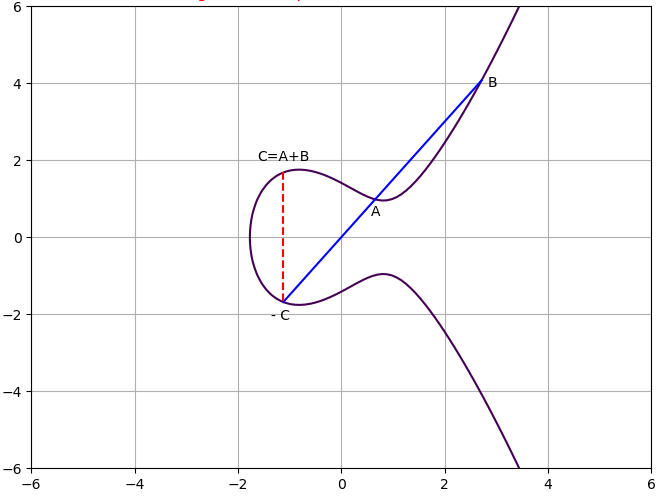
\includegraphics[width=\textwidth, valign=c]{sum_a_b_ec_p3_1.png}
        \caption{Caso generale}
    \end{minipage}
    \hfill
    \begin{minipage}[t]{0.45\textwidth}
        \centering
        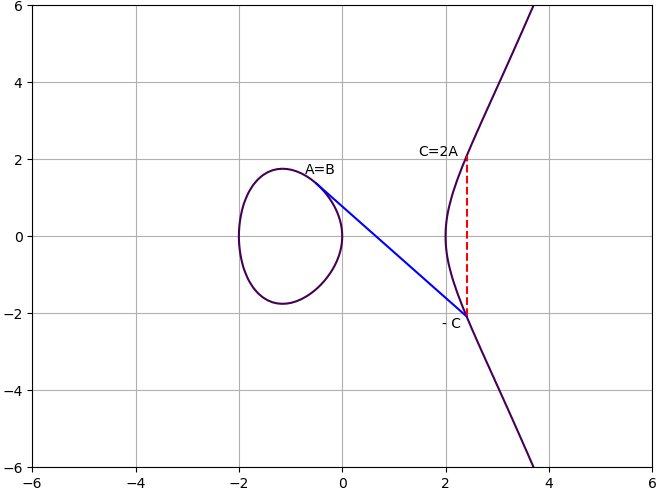
\includegraphics[width=\textwidth, valign=c]{sum_a_b_ec_p2_2.png}
        \caption{Caso di punti coincidenti}
    \end{minipage}
    \begin{minipage}[t]{0.45\textwidth}
        \centering
        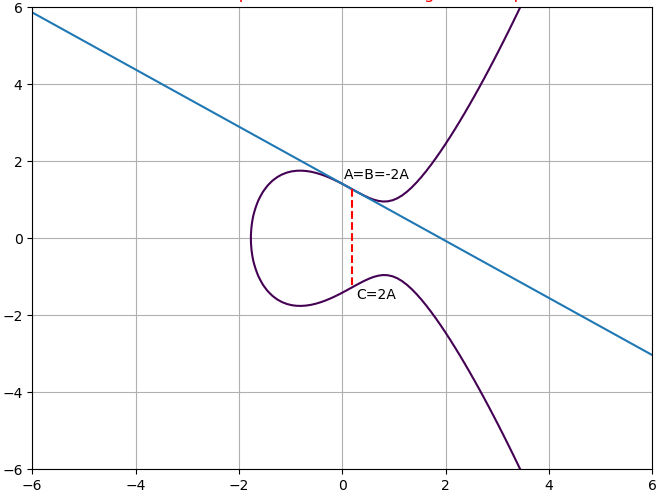
\includegraphics[width=\textwidth, valign=c]{sum_a_b_ec_p1_3.png}
        \caption{Caso di punto con flesso}
    \end{minipage}
    \hfill
    \begin{minipage}[t]{0.45\textwidth}
        \centering
        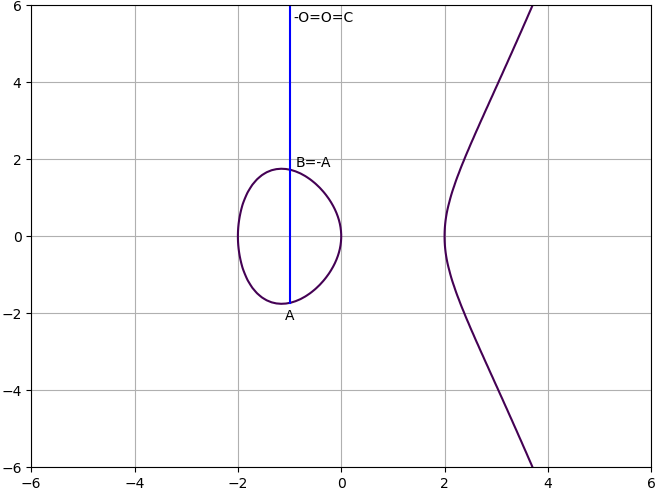
\includegraphics[width=\textwidth, valign=c]{sum_a_b_ec_p2_1.png}
        \caption{Caso retta verticale}
    \end{minipage}
\end{figure}
I punti sulla curva elittica con operazione di addizione appena definita formano un gruppo \textbf{abelliano}, ovvero un gruppo dove è definita la proprietà \textbf{commutativa}. Il gruppo generato mantiene anche la proprietà di \textbf{associazione} rispetto alla somma di punti. 
\begin{enumerate}
    \item \textbf{Chiusura}, in forza anche dell'introduzione del punto $\mathcal{O}$.
    \begin{itemize}
        \item i casi in cui i due punti sono diversi da $\mathcal{O}$ sono definiti geometricamente nelle \textit{Figure 6.16, 6.17, 6.18} in tutti i casi $A + B$ è ancora un punto della curva (eventualmente $\mathcal{O}$).
        \item $\mathcal{O} + \mathcal{O} = \mathcal{O}$, infatti per la proprietà del \textbf{punto all'infinito} sappiamo che $\mathcal{O}$ ha molteplicità 3 e che quindi la terza intersezione è $\mathcal{O}$, ma anche il suo \textbf{simmetrico}.
        \item $A + \mathcal{O} = A$.
    \end{itemize}
    \item $\mathcal{O}$ è l'elemento \textbf{neutro}: $A + \mathcal{O} = \mathcal{O} + A = A$
    \item ogni elemento \textit{A} ha un opposto, precisamente il punto di simmetria sulla curva \textit{-A}, infatti $A + (-A) = \mathcal{O}$.
    \item la proprietà \textbf{associativa} è verificata.
    \item la proprietà \textbf{commutativa} è verificabile geometricamente in quanto la retta che passa per due punti è individuabile indipendentemente dall'ordine dei punti.
\end{enumerate}
\   \\
\textbf{Caso A $\neq$ B} \\
Noti i punti $A(x_a, y_a) \text{ e } B(x_b, y_b)$ che sono soluzioni per il sistema:
\begin{center}
    \begin{math}
        \begin{cases}
            y^2 = x^3 + ax + b \\
            y = mx + q
        \end{cases}
        \Rightarrow R = 
        \begin{cases}
            y = y_a = y_b \qquad \text{ se } m = 0 \\
            y = (\frac{y_b - y_a}{x_b - x_a})x + (y_a - (\frac{y_b - y_a}{x_b - x_a}) \cdot x_a)
        \end{cases}
    \end{math}
\end{center}
$$\Rightarrow (mx + q)^2 = x^3 + ax + b \Rightarrow x^3 - mx^2 + (a - 2mq)x + b - q^2 = 0$$
Siccome due soluzione le conosciamo già e sappiamo che sono $A(x_a, y_a) \text{ e } B(x_b, y_b)$, possiamo visualizzare le \textit{x} del polinomio di terzo grado come: $(x - x_a)(x - x_b)(x - x_{\overline{c}}) = 0$ a noi interessa trovare il punto $-C(x_{\overline{c}}, y_{\overline{c}})$ che intersechi la curva \textit{E} appartente alla retta descritta da \textit{A} e \textit{B}.
\begin{center}
    \begin{math}
        \begin{aligned}
            (x - x_a)(x - x_b)(x - x_c) &= 0 \\
            x^3 - mx^2 + (a - 2mq)x + b - q^2 &= 0 \\
            (x - x_a)(x - x_b)(x - x_c) &= x^3 - mx^2 + (a - 2mq)x + b - q^2 \\
            x^3 + x^2 \cdot (- x_a - x_b - x_c) + x \cdot (x_a x_b + x_a x_c + x_b x_c) + x_a x_b x_c &= x^3 - mx^2 + (a - 2mq)x + b - q^2
        \end{aligned}
    \end{math}
\end{center}
Ugualiando i coefficienti di grado \textit{2} avremo: $-m^2 = - x_a - x_b - x_c$ e quindi potremo trovare la coordianta del punto $-C(x_{\overline{c}}, y_{\overline{c}}) = (m^2 - x_a - x_b, m \cdot x_{\overline{c}} + q)$. Il punto somma $C = A + B = -(-C)$ e siccome abbiamo detto che la \textbf{EC} è simmetrica rispetto all'asse delle \textit{x} avremo che $x_{\overline{c}} = x_c$ e $y_{\overline{c}} = -y_c$ andando così a descrivere il punto $C(x_c, y_c)$.
\\ \newline
\textbf{Caso A = B} \\
Quando i due punti coincidono è necessario calcolare il \textbf{coefficente angolare \textit{m}} della retta $R_A$ tangente alla curva per il punto \textit{A}. Anche se la curva non è definita in maniera esplicita è possibile rappresentarla come l'unione dei graifici di due funzioni, più precisamente:
$$y_1(x) = \sqrt{x^3 + ax + b} \;\;\; \cup y_2(x) = - \sqrt{x^3 + ax + b}$$
Dobbiamo quindi calcolare la derivata $\frac{d}{dx}y_1(x')$ e $\frac{d}{dx}y_2(x')$ dove $(x', y')$ è un punto definito sulla curva $y_1 \text{ se } y' \geq 0$, quindi vale $y_1(x') = y'$ mentre invece è definito sulla curva $y_2 \text{ se } y' \leq 0$, quindi vale $y_2(x') = y'$ possiamo calcolare i coefficienti delle rette tangenti:
\begin{center}
    \begin{math}
        \begin{aligned}
        \frac{d}{dx}y_1(x') &= \frac{3x'^2 + a}{2\sqrt{x'^3 + ax' + b}} = \frac{3x'^2 + a}{2y_1(x')} =& \frac{3x'^2 + a}{2y'} \\
        \frac{d}{dx}y_2(x') &= - \frac{3x'^2 + a}{2\sqrt{x'^3 + ax' + b}} = - \frac{3x'^2 + a}{2(- y_2(x'))} = - \frac{3x'^2 + a}{-2y'} =& \frac{3x'^2 + a}{2y'}
        \end{aligned}
    \end{math}
\end{center}
Avremo quindi che il calcolo del \textbf{coefficente angolare} è \textcolor{blue}{$m = \frac{3x'^2 + a}{2y'}$}. \\
Pseudo-codice per il calcolo di \textbf{C = A + B}:
\begin{lstlisting}[label=lst:rho-polland, basicstyle=\small, mathescape=true]
def sumPointOnEC(A: point, B: point) -> point:
    if A = = $\mathcal{O}$: return B
    if B = = $\mathcal{O}$: return A
    if B = = -A: return $\mathcal{O}$

    if $A \neq B$: m = $\frac{y_b - y_a}{x_b - x_a}$
    if $A == B$: m =  $\frac{3x_a^2 + a}{2y_a}$
        
    # C(x, y)
    return point($m^2 - x_a - x_b$, $- (mx_c + q)$)
\end{lstlisting}

\section{Curve in $\mathbb{Z}_p$}
Indicheremo una curva elittica a coefficienti \textit{a} e \textit{b}, definita sul campo $\mathbb{Z}_p$, usando la notazione $E_{a,b}(\mathbb{Z}_p)$.
\begin{figure}[h]
    \centering
    \begin{minipage}[t]{0.45\textwidth}
        \centering
        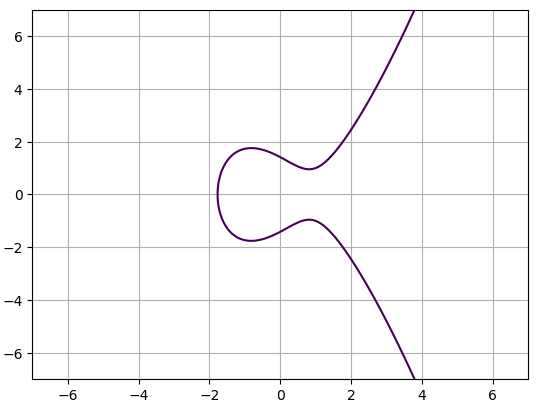
\includegraphics[width=\textwidth, valign=c]{ec_liscia_2.png}
        \caption{$E_{(-2, -2)}$}
    \end{minipage}
    \hfill
    \begin{minipage}[t]{0.45\textwidth}
        \centering
        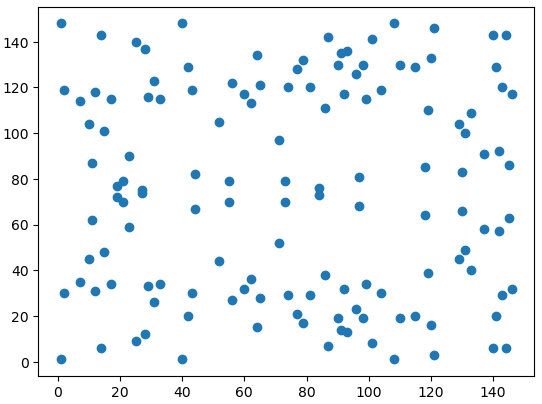
\includegraphics[width=\textwidth, valign=c]{ec_liscia_2_zp.png}
        \caption{$E_{-2, 2}(\mathbb{Z}_{149})$}
    \end{minipage}
\end{figure}
\   \\
Anche se, come possiamo notare, la geometria qui non ci può aiutare, i risultati algebrici rimangono ancora validi. Se un'equazione cubica (a coefficienti in $\mathbb{Z}_p$) ha due radici in $\mathbb{Z}_p$, allora ha anche la terza radice in $\mathbb{Z}_p$. Questo consenti di definire l'operazione di addizione come nel caso reale. Analogamente a quanto fatto per il gruppo $\mathbb{Z}_p^*$, possiamo definire dei \textbf{sottogruppi ciclici} dei punti $S_{E_{a,b}}(\mathbb{Z}_p)$. Il sottogruppo generato da un punto $g(x_g, y_g)$ è definito nel seguente modo:
\begin{center}
    \begin{math}
        S_{E_{a,b}(\mathbb{Z}_p)}(g)=\{a\in E_{a,b}(\mathbb{Z}_p)|\exists k\geq0, a = k\cdot g = \underbrace{g+g+\ldots+g}_{k-1\ \mathrm{somme}}\}
    \end{math}
\end{center}
L'operazione $k\cdot g$, dove $k$ è un intero non negativo e $g$ è un punto sulla curva, è detta \textbf{\textit{moltiplicazione scalare}}. Normalmente il gruppo dei punti sulla curva \textbf{non è ciclico}, per esso vale il teorema di \textbf{\textit{lagrange}}, ma non quello fondamentale dei gruppi ciclici.
\\ \newline
\textbf{Logaritmo Discreto su Curva Elittica} \\
Se \textit{g} è un punto sulla curva $S_{E_{a,b}(\mathbb{Z}_p)}$ che genera l'intero gruppo (quindi \textit{g} è una \textbf{radice primitiva} di $S_{E_{a,b}(\mathbb{Z}_p)}$), allora per ogni altro punto $z \in S_{E_{a,b}(\mathbb{Z}_p)} \rightarrow \exists k \geq 0 \; | \; z = k \cdot g$. Il minimo intero \textit{k} che soddisfa questa ugualianza è il \textbf{logaritmo a base \textit{g} di \textit{z}} rappresentabile nella forma $k = \log_{g}{z}$. Da un punto di vista computazionale, dati \textit{k} e \textit{g} è facile trovare il valore di \textit{z}, infatti l'algoritmo segue lo stesso schema dell'esponenziale modulare, ovvero il \textbf{\textit{Recursive Doubling}}. Il calcolo di \textit{z} parte dalla rappresentazione binaria di \textit{k} accumulando le quantità solo in corrispondenza degli \textit{1} della rappresentazione binaria di \textit{k}, il calcolo inverso, ovvero dati \textit{g} e \textit{z} trovare \textit{k} è invece \textbf{computazionalemente difficile} e non sono noti algoritmi con costo polinomiale. \\
Date le proprietà presenti del gruppo $E_{a,b}(\mathbb{Z}_p)$ è quindi facile immaginare del perché le \textbf{EC} abbiamo suscitato un tale interesse nell'ambito della crittografia. È però interessante osservare la questione dei \textbf{numeri di punti sulla curva}, infatti questo è l'\textbf{ordine} del nostro gruppo $E_{a,b}(\mathbb{Z}_p)$, quando si lavorava su gruppo $\mathbb{Z}_p^*$ l'ordine veniva facilmente calcolato dalla quantità $p - 1$ e quindi si potevano prendere delle precauzioni per evitare che i sottogruppi di $\mathbb{Z}_p^*$ avessero un ordine molto piccolo, grazie al \textbf{teorema di Lagrange} e la diretta costruzione del primo del tipo $p = 2q + 1$ dove anche \textit{q} fosse un numero primo. In questo modo si poteva controllare l'ordine dei sottogruppi di $\mathbb{Z}_p^*$ e quindi tenerli controllati in modo da evitare che fossero fattori semplici di \textit{p} (concetto dei \textbf{safe prime}). Nel caso delle \textbf{EC} non abbiamo un ``teorema'' che ci possa guidare alla scelta dei parametri \textit{a, b, p} in modo da controllare le dimensioni del gruppo dei punti sulla curva. 
\\ \newline
\textbf{Numeri di Punti sulla Curva}: se \textit{p} è il modulo, il numero di punti su una curva può superare il valore di $2p + 1$ questo perché se $x^3 + ax + b \bmod p \neq 0$ è un residuo quadratico, allora al valore \textit{x} corrispondono due radici in \textit{p} e quindi \textbf{due punti sulla curva}. Tuttavia per raggiungere il limite $2p + 1$ è necessario che $x^3 + ax + b$ sia un residuo quadratico modulo $p \; \forall x \in \{0, 1, ..., p - 1\}$ è però ragionevole attendersi che circa metà dei valori siano residui quadrati e metà residui non-quadratici in questo modo il numero di punti torna ad essere circa \textit{p}. Il numero di punti su una curva viene rappresentato da: $\#E(a, b, p)$. \\
Il \textbf{\textit{Teorema di Hasse}} fornisce un \textit{bound} più preciso:
\begin{center}
    $|\#E(a, b, p) - (p + 1)| \leq 2\sqrt{p}$
\end{center}
Dal punto di vista algoritmico, il miglior risultato noto per determinare il numero ``esatto'' di punti è dovuto a \textbf{\textit{\href{http://www.numdam.org/item/JTNB_1995__7_1_219_0.pdf}{René Schoof}}} la cui versione non ottimizzata dell'algoritmo ha complessità $\mathcal{O}((\log{p})^8)$ va però tenuto presente che per ogni curva l'algoritmo va eseguito una sola volta. In generale è sconsigliato cercare delle \textbf{safe curves} in autonomia, esistono già dei database in cui vengono salvate curve ritenute sicure (https://safecurves.cr.yp.to/).